\documentclass[10pt]{article}
\usepackage{extsizes}
\usepackage[affil-it]{authblk}
\usepackage[T1]{fontenc}
\usepackage[utf8]{inputenc}
\usepackage[italian]{babel}
\usepackage{amsfonts}
\usepackage{amsmath}
\usepackage{amsthm}
\newtheorem{thm}{Teorema}
\usepackage{graphicx}
\usepackage{subfigure}
\usepackage{enumitem}
\usepackage{amssymb}
\usepackage{cancel}
\usepackage{hyperref}
\usepackage{listings}
\usepackage{color}
\usepackage{algpseudocode,algorithm,algorithmicx}


\definecolor{codegreen}{rgb}{0,0.6,0}
\definecolor{codegray}{rgb}{0.5,0.5,0.5}
\definecolor{codepurple}{rgb}{0.58,0,0.82}
\definecolor{backcolour}{rgb}{0.95,0.95,0.92}

\usepackage{listings} %For code in appendix
\lstset
{ %Formatting for code in appendix
	backgroundcolor=\color{backcolour},   
    commentstyle=\color{codegreen},
    keywordstyle=\color{magenta},
    numberstyle=\tiny\color{codegray},
    stringstyle=\color{codepurple},	
	frame=tb
    language=Python,
    basicstyle=\footnotesize,
    numbers=left,
    stepnumber=1,
    showstringspaces=false,
    tabsize=1,
    breaklines=true,
    breakatwhitespace=false,
}

\usepackage[explicit]{titlesec}
\usepackage{xkeyval}
\usepackage{tikz}
\usetikzlibrary{tikzmark,calc}
\usepackage{lipsum}

\newlength\LeftSep
\newlength\RightSep
\newlength\TitleWd
\newlength\VertLineWd
\newlength\SpaceBefore
\newlength\SpaceAfter
\newlength\RuleAddition
\newcommand\SectionFont{\normalfont\Large\bfseries}
\newsavebox\TitleBox
\newcounter{tmp}

\setlength\LeftSep{\marginparsep}
\setlength\RightSep{\marginparsep}
\setlength\TitleWd{0.6666\textwidth}
\setlength\VertLineWd{1pt}
\setlength\SpaceBefore{3.5ex plus 1ex minus .2ex}
\setlength\SpaceAfter{2.3ex plus .2ex}
\setlength\RuleAddition{0pt}

\makeatletter
\define@key{fctaylor}{leftsep}{\setlength\LeftSep{#1}}
\define@key{fctaylor}{rightsep}{\setlength\RightSep{#1}}
\define@key{fctaylor}{titlewidth}{\setlength\TitleWd{#1}}
\define@key{fctaylor}{verticalrulewidth}{\setlength\VertLineWd{#1}}
\define@key{fctaylor}{spacebefore}{\setlength\SpaceBefore{#1}}
\define@key{fctaylor}{spaceafter}{\setlength\SpaceAfter{#1}}
\define@key{fctaylor}{sectionfont}{\renewcommand\SectionFont{#1}}
\define@key{fctaylor}{ruleaddition}{\setlength\RuleAddition{#1}}

\newcommand\FCsectionformat[1][]{%
\setkeys{fctaylor}{#1}
\titleformat{\section}
  {\SectionFont}{}{0em}
  {%
    \parbox[t]{1em}{\thesection}\hspace{\LeftSep}%
    \stepcounter{tmp}%
    \tikz[remember picture]
      \draw[overlay,line width=\VertLineWd] 
        ([xshift=-\RightSep,yshift=\dimexpr\ht\strutbox+\RuleAddition\relax]pic cs:start-\thetmp) -- 
        ( $ ({pic cs:start-\thetmp}|-{pic cs:end-\thetmp}) + (-\RightSep,\dimexpr+\ht\strutbox-\baselineskip-\RuleAddition\relax)$ );%
    \hspace{\RightSep}% 
    \parbox[t]{\TitleWd}{%
      \SectionFont\raggedright\strut%
      \tikzmark{start-\thetmp}##1\tikzmark{end-\thetmp}\strut}%
  }
\titleformat{name=\section,numberless}
  {\SectionFont}{}{0em}
  {%
   \hspace*{\dimexpr1em+\LeftSep\relax}%
    \stepcounter{tmp}%
    \tikz[remember picture]
      \draw[overlay,line width=\VertLineWd] 
        ([xshift=-\RightSep,yshift=\dimexpr\ht\strutbox+\RuleAddition\relax]pic cs:start-\thetmp) -- 
        ( $ ({pic cs:start-\thetmp}|-{pic cs:end-\thetmp}) + (-\RightSep,\dimexpr+\ht\strutbox-\baselineskip-\RuleAddition\relax)$ );%
    \hspace{\RightSep}% 
    \parbox[t]{\TitleWd}{%
      \SectionFont\raggedright\strut%
      \tikzmark{start-\thetmp}##1\tikzmark{end-\thetmp}\strut}%
   }
}
\titlespacing*{\section}
  {0pt}{\SpaceBefore}{\SpaceAfter}
\titlespacing*{name=\section,numberless}
  {0pt}{\SpaceBefore}{\SpaceAfter}
\makeatother

\FCsectionformat

\usepackage{titling}


\title{Progetto di Tecnologie del Linguaggio Naturale:\\Esercizio 1}
\date{}
\author{Paolo Didier Alfano}
\affil{Università degli Studi di Torino}

\begin{document}
\maketitle

\begin{abstract}
	L'esercizio prevede l'implementazione di un traduttore diretto dalla lingua italiana a quella inglese. La costruzione del traduttore si articola in due fasi: nella prima forniamo un'implementazione dell'algoritmo di Viterbi. Nella seconda, mediante un sistema di regole, effettuiamo la traduzione diretta a cui segue una breve analisi dei risultati ottenuti. Concludiamo con una breve appendice che mostra l'esito di un semplice esperimento di machine learning inerente il PoS tagging.
\end{abstract}

\section{Strutture dati di maggior rilievo}
Prima di procedere nello studio degli algoritmi, andiamo ad analizzare velocemente le strutture dati utilizzate:
\begin{itemize}
	\item Dizionari: nel corso del progetto abbiamo utilizzato tre dizionari
	\begin{itemize}
		\item[-] \texttt{posDictionary}: associa ad ognuno dei diciassette possibili PoS tag un valore numerico in base ad un ordinamento lessicografico degli stessi. Questo dizionario viene utilizzato per semplificare le operazioni di indicizzazione sulle matrici dell'algoritmo di Viterbi.
		\item[-] \texttt{reverseDictionary}: similmente, questo dizionario associa ad ogni numero da zero a sedici un corrispondente PoS tag. Anche questo dizionario viene utilizzato per facilitare le operazioni di indicizzazione.
		\item[-] \texttt{itaEngDict}: contiene le traduzioni dei vocaboli dall'italiano all'inglese. Viene utilizzato nella parte finale del progetto per effettuare la traduzione diretta
	\end{itemize}
	
	\item \texttt{wordsArray}: matrice formata da due colonne e da un numero di righe pari alla cardinalità del training set. La riga i-esima della matrice contiene l'i-esimo vocabolo, e il PoS tag associato all'i-esimo vocabolo.
	
	\item \texttt{wordStructure}: matrice che ha un numero di righe pari alla cardinalità dell'insieme di parole utilizzate nel training set e che ha tante colonne quanto il numero di PoS tag possibili. Indica per ognuna delle parole, quante volte tale parola è occorsa come ognuno dei possibili PoS tag.
	
	\item \texttt{emissionMatrix}: matrice di emissione per la frase che stiamo analizzando. Supponendo di avere una frase composta da $n$ vocaboli, otterremo una matrice di emissione di dimensione $p \times n$ dove $p$ è la cardinalità dell'insieme dei PoS tag.
	
	\item \texttt{viterbiMatrix}: matrice utilizzata dall'algoritmo di Viterbi. Anche in questo caso la dimensione della matrice è $p \times n$ dove $p$ è la cardinalità dell'insieme dei PoS tag mentre $n$ è il numero di vocaboli che compongono la frase da analizzare
	
	\item \texttt{backpointerMatrix}: matrice utilizzata dall'algoritmo di Viterbi per tenere traccia dei puntatori all'indietro. Anche in questo caso la dimensione della matrice è $p \times n$ dove $p$ è la cardinalità dell'insieme dei PoS tag mentre $n$ è il numero di vocaboli che compongono la frase da analizzare
	
	\item \texttt{wordsMostFreqUse}: matrice a due colonne contenente per ogni parola del training set, il suo utilizzo più comune. Dunque la riga i-esima della matrice possiede due elementi: il primo è l'i-esimo vocabolo, il secondo è il tag associato più di frequente all'i-esimo vocabolo.
	
	\item \texttt{translated}: array contenente i vocaboli tradotti mediante il processo di traduzione diretta.
\end{itemize}

\section{L'algoritmo di Viterbi}
\subsection{Implementare l'algoritmo di Viterbi}
Per implementare l'algoritmo di Viterbi abbiamo dovuto effettuare alcune operazioni preliminari.\\
Innanzitutto abbiamo costruito i due dizionari \texttt{posDictionary} e\\
\texttt{reverseDictionary}, mediante alcuni comandi della forma:
\begin{lstlisting}[language=Python]
posDictionary['ADJ'] = 0
...
reverseDictionary['0'] = 'ADJ'
\end{lstlisting}
In questo caso abbiamo specificato che il dizionario in presenza di un aggettivo "ADJ" deve fornire in output il valore 0. Come dicevamo i dizionari ci serviranno per le operazioni di indicizzazione nella matrice dell'algoritmo di Viterbi.\\
Successivamente abbiamo dovuto creare il vettore \texttt{tagStart} contenente le probabilità\\
\\
$P(t_0 | start)$\\
\\
dove $start$ è lo stato iniziale fittizio dell'algoritmo di Viterbi. Di fatto \texttt{tagStart} è un array contenente le probabilità di transire dallo stato iniziale ad ogni PoS tag possibile. Ad esempio \texttt{tagStart[0]}\footnote{Ricordiamo che le celle sono ordinate lessicograficamente sui PoS tag. Dunque le celle conterranno rispettivamente:\\ 'ADJ', 'ADP', 'ADV', 'AUX', 'CCONJ', 'DET', 'INTJ', 'NOUN', 'NUM', 'PART', 'PRON', 'PROPN', 'PUNCT', 'SCONJ', 'SYM', 'VERB', 'X'} contiene la probabilità che il primo elemento di una frase sia un aggettivo.\\
Per calcolare i valori contenuti all'interno di questo array abbiamo valutato quale fosse il PoS tag dopo ogni elemento di punteggiatura in tutto il training set.\\
Il risultato, ottenuto su un totale di 40.718 elementi di punteggiatura, indica che l'elemento più frequente all'inizio di una frase è l'articolo, che occorre nel $18\%$ dei casi.\\
Successivamente abbiamo costruito la matrice \texttt{tagConjCount} che valuta quanto di frequente un certo tag in posizione $i$ sia preceduto da un qualunque altro tag in posizione $i-1$. Dunque la matrice \texttt{tagConjCount} è formata da diciassette righe e altrettante colonne.\\
\\
Allo stesso tempo abbiamo anche calcolato i valori del vettore \texttt{tagCount} che conta il numero di occorrenze di ogni PoS tag nel training set.\\
\\
In seguito abbiamo definito la funzione \texttt{buildEmission} che costruisce la matrice di emissione per la frase da studiare. Come da specifica, la matrice di emissione ha la stessa dimensione della matrice utilizzata nell'algoritmo di Viterbi. Dunque questa matrice possiede tante righe quanti sono i PoS tag possibili, e tante colonne quante sono le parole che compongono la frase da analizzare.\\
La funzione procede per ogni parola a verificarne la presenza nel training set e va a contare quante volte ogni PoS tag viene associato a quella parola. In seguito andiamo a normalizzare i valori.\\
Qualora una certa parola non occorra nel training set, tutte le celle della colonna relativa a tale parola conterranno un valore pari al rapporto $\dfrac{1}{\#PoS\ tag}$, ovvero pari a $\dfrac{1}{17}$.\\
\\
A questo punto abbiamo potuto finalmente definire la funzione relativa all'algoritmo di Viterbi, detta  \texttt{viterbiAlgorithm}. La funzione riceve in input la frase da analizzare l'insieme dei PoS tag possibili. In base a queste indicazioni va ad eseguire i passi ben noti dell'algoritmo di Viterbi:

\begin{lstlisting}[language=Python]
def viterbiAlgorithm(phrase, posSet):
    viterbiMatrix = np.zeros((len(posSet), len(phrase)))
    backpointerMatrix = np.zeros((len(posSet), len(phrase)))
    emissionMatrix = buildEmission(phrases[p], posSet)
    
    #Initialization step
    for i in range(0, len(posSet)):
        viterbiMatrix[i][0] = tagStart[i] * emissionMatrix[0][i]
          
    #Recursion step
    for i in range(1, len(phrase)):
        for j in range(0, len(posSet)):
            maxProb = -1
            maxIndex = -1
            for k in range(0, len(posSet)):
                currentProb = viterbiMatrix[k][i-1] * tagCondProb[j][k] * emissionMatrix[i][j]
                
                if(currentProb>maxProb):
                    maxProb = currentProb
                    maxIndex = k
            viterbiMatrix[j][i]=maxProb
            backpointerMatrix[j][i] = maxIndex
          
    return [viterbiMatrix, backpointerMatrix]
\end{lstlisting}

Il codice è strutturato come segue: le righe 2, 3 e 4 costruiscono le matrici necessarie al funzionamento. Successivamente con le righe 7 e 8 andiamo ad assegnare i valori alla prima colonna della matrice di Viterbi. Le linee successive alle 9 mostrano invece i passi della ricorsione dell'algoritmo di Viterbi. Per calcolare ognuna delle probabilità della matrice di Viterbi consideriamo le tre seguenti quantità:
\begin{itemize}
	\item[-] viterbiMatrix[k][i-1]: il valore della matrice alla colonna precedente $i-1$ in corrispondenza del tag corrente $k$
	\item[-] tagCondProb[j][k]: la probabilità che al tag $j$ segua il tag $k$
	\item[-] emissionMatrix[i][j]: la matrice di emissione per la parola $i$ relativamente al tag $j$
\end{itemize}

\noindent L'ultima funzione che abbiamo specificato è la funzione \texttt{viterbi} che serve per mettere insieme le varie parti e per permettere una facile esecuzione dell'algoritmo a un più alto livello.\\
Infatti la funzione \texttt{viterbi} necessita semplicemente di due argomenti
\begin{itemize}
	\item[-] phrases: array di frasi su cui vogliamo eseguire l'algoritmo
	\item[-] posSet: l'insieme dei possibili PoS tag
\end{itemize}
In base a questi due argomenti eseguiremo la funzione \texttt{viterbiAlgorithm} per ognuna delle frasi contenute in phrases cercando di classificare ogni parola di tali frasi con i PoS tag contenuti in posSet.\\
\\
Successivamente abbiamo introdotto il codice necessario al calcolo della baseline. Per ogni parola nel test set andiamo a verificare se è presente nel training set. Nel caso in cui sia presente associamo a tale parola il PoS tag con cui compare più frequentemente. Se invece tale parola non è mai comparsa nel training set, gli assegniamo  il PoS tag occorso più di frequente nel training set, ovvero il PoS tag NOUN. Dunque tutte le parole non occorse nel training set vengono considerati nomi.

\subsection{Risultati ottenuti}
Andiamo a considerare i risultati della nostra implementazione dell'algoritmo di Viterbi e quelli ottenuti dalla baseline.\\
Andando a suddividere il test set in frasi, abbiamo ottenuto 670 frasi.\\
L'accuratezza ottenuta dall'algoritmo di Viterbi su tale test set è pari a 
\begin{equation}
	acc_{viterbi}= 0.913
\end{equation}
Il tempo medio di esecuzione\footnote{Calcolato in base a trenta esecuzioni dell'algoritmo. Dunque non pretendiamo di avere alcuna valenza statistica, ma solo di fornire un ordine di grandezza al lettore} su questo test set si è attestato intorno al valore
\begin{equation}
	t_{viterbi}= 30.29 s
\end{equation}
questo significa che l'algoritmo di Viterbi impiega mediamente $0.04$ secondi per assegnare i PoS tag a frasi composte mediamente da $30$ parole\footnote{La lunghezza media di una frase è stata ottenuta dividendo il numero di parole nel test set, pari a 20254, per il numero di frasi, pari a 670.}.\\
\\
Il valore di accuratezza di baseline è in linea con quanto riportato in letteratura:
\begin{equation}
	acc_{baseline} = 0.892
\end{equation}

\section{Traduzione diretta}
Una volta ottenuti i corretti PoS tag per le frasi, abbiamo lavorato sul procedimento di traduzione diretta. Per farlo abbiamo costruito il dizionario \texttt{itaEngDict}.\\
Per effettuare al meglio il procedimento di traduzione, il dizionario contiene le parole da tradurre a cui abbiamo concatenato un identificativo numerico. L'identificativo numerico serve in quei casi in cui una certa parola in italiano può avere più traduzioni in inglese a seconda del contesto in cui si trova. Ad esempio:
\begin{lstlisting}[language=Python]
itaEngDict['la0'] = 'of'
itaEngDict['la1'] = 'it'
\end{lstlisting}
Con questo intendiamo dire che di default la parola italiana 'la' verrà tradotta con la parola inglese 'of'. In certi casi invece, tale parola deve essere tradotta con la parola inglese 'it'. A seconda del contesto in cui siamo, concateneremo uno 0 o un 1 alla parola da tradurre per ottenere la traduzione desiderata.\\
\\
Per stabilire quale traduzione sia consona per una certa parola, abbiamo sviluppato un sistema di regole\footnote{Simulate mediante degli statement if} all'interno della funzione \texttt{invertingPosRules}. Questa funzione, riceve in input i seguenti argomenti
\begin{itemize}
	\item[-] phrase: la frase da tradurre
	\item[-] posTagArray: array che contiene i tag associati alla frase da tradurre
	\item[-] i: la posizione corrente che indica quale parola di phrase dovremo andare a tradurre direttamente
	\item[-] translated: array che contiene le parole già tradotte. Tali parole devono essere disponibili anche in seguito perché alcune situazioni, come l'introduzione di un genitivo sassone, potrebbero andare a effettuare inserimenti non solo in coda ma anche in mezzo a parole tradotte in precedenza
\end{itemize}
La funzione va ad eseguire una serie di controlli che permettono di gestire alcune situazioni particolari, come l'inversione di un nome con un aggettivo, oppure l'introduzione di un genitivo sassone.\\
Nella maggior parte dei casi non dobbiamo gestire situazioni particolari, e dunque possiamo andare a tradurre parola per parola. Quando invece abbiamo delle situazioni più complesse, potrebbe capitare di dover tradurre più di una parola con una sola iterazione della funzione \texttt{invertingPosRules}. Per far fronte a questa situazione, la funzione \texttt{invertingPosRules} restituisce il numero di parole che sono state tradotte con la chiamata corrente. Per comprendere meglio quanto appena detto, riportiamo il codice di seguito:
\begin{lstlisting}[language=Python]
def invertingPosRules(phrase, posTagArray, i, translated):
			#Invert noun and adjective("mossa leale" --> "fair move")
    if(i<len(phrase)-1):
        if((posTagArray[i]=='NOUN') & (posTagArray[i+1]=='ADJ')):
            translated.append(itaEngDict[phrase[i+1]+'0'])
            translated.append(itaEngDict[phrase[i]+'0'])
            return 2
            
    #Handle Saxon genitive
    if((i<len(phrase)-2) & (i>0)):
        if((posTagArray[i]=='ADP') & (posTagArray[i+1]=='DET') & (posTagArray[i+2]=='NOUN')):
            j=i-1
            while(posTagArray[j] == 'NOUN'): 
                j-=1
            translated.insert(j+1, itaEngDict[phrase[i+1]+'0'])
            translated.insert(j+2, itaEngDict[phrase[i+2]+'0'])
            translated.insert(j+3, itaEngDict[phrase[i]+'1'])
            return 3
        
    # Handle subject's Saxon genitive("E' la" --> "It's")  
    if(i<len(phrase)-1):
        if((posTagArray[i]=='AUX') & (posTagArray[i+1]=='DET')):
            translated.append(itaEngDict[phrase[i+1]+'1'])
            translated.append(itaEngDict[phrase[i]+'1'])
            return 2
    
    translated.append(itaEngDict[phrase[i]+'0'])
    return 1
\end{lstlisting}
Consideriamo ad esempio la gestione dell'inversione tra nome e aggettivo(che utilizziamo per tradurre correttamente "mossa leale" in "fair move"). Questa inversione viene gestita dalla riga 3 alla riga 7 del codice appena illustrato.\\
Lo statement if alla riga 3 controlla semplicemente che non abbiamo raggiunto il fondo della frase, ovvero che dopo la parola corrente ve ne sia ancora un'altra con cui faremo eventualmente l'inversione. Lo statement if alla riga 4 controlla invece che la parola corrente sia un nome, e che la parola successiva sia un aggettivo.\\
Se si verificano le due condizioni appena descritte, andiamo prima a tradurre l'aggettivo(riga 5) e inseriamo la traduzione nel vettore contenente le parole già tradotte. In seguito andiamo a tradurre il nome(riga 6) e lo inseriamo subito dopo l'aggettivo. In questo modo abbiamo effettuato l'inversione tra nome e aggettivo. Notiamo che con questa iterazione della funzione abbiamo tradotto due parole in modo diretto. Dunque la funzione restituisce il valore 2.\\ 
Consideriamo infine, il caso in cui nessuna delle regole è applicabile. In tal caso la funzione va a tradurre solo la parola corrente in modo diretto e restituisce il valore 1 ad indicare che soltanto una parola è stata tradotta.\\
\\
Per operare effettivamente la traduzione abbiamo sviluppato una funzione\\ \texttt{translatePhrase} che presa una frase e l'array dei suoi PoS tag, opera come segue

\begin{lstlisting}[language=Python]
def translatePhrase(phrase, posTagArray):
    translated = []
    i=0
    while(i<len(phrase)):
        incr=invertingPosRules(phrase,posTagArray,i,translated)
        i+= incr
    return translated
\end{lstlisting}

\noindent Dunque viene eseguita la funzione \texttt{invertingPosRules} che effettua la traduzione e ci restituisce quante parole sono state tradotte con la sua chiamata. In base al valore restituito andremo poi a incrementare l'indice che scorre le parole della frase da tradurre.\\
\\
Le frasi da tradurre erano 
\begin{itemize}
	\item[-] È la spada laser di tuo padre
	\item[-] Ha fatto una mossa leale
	\item[-] Gli ultimi avanzi della vecchia Repubblica sono stati spazzati via
\end{itemize}

\noindent La traduzione ottenuta mediante gli algoritmi appena descritti è la seguente

\begin{itemize}
	\item[-] it's your father's saber light 
	\item[-] he made a fair move 
	\item[-] the last remnants of old republic have been swept away
\end{itemize}

\noindent Come è possibile osservare, la traduzione ottenuta è buona e mostra una corretta gestione delle due situazioni più problematiche: l'introduzione del genitivo sassone e l'inversione dei nomi con gli aggettivi.

\section{Conclusioni}
Nelle scorse pagine abbiamo visto una possibile implementazione dell'algoritmo di Viterbi. L'accuratezza ottenuta mediante l'algoritmo è superiore, seppur non di troppo, al valore di baseline.\\
Riteniamo che il risultato ottenuto sia soddisfacente considerando che, oltre al buon valore di accuratezza ottenuto, l'esecuzione dell'algoritmo sull'intero test set richiede un tempo essenzialmente breve.\\
\\
Per quanto riguarda la traduzione diretta, mediante un semplice sistema di regole basato su statement if, abbiamo ottenuto una buona traduzione delle frasi, dunque possiamo ritenerci soddisfatti.

\newpage

\section{Appendice: un esperimento di machine learning}
Parallelamente allo sviluppo dell'algoritmo di Viterbi è stato sviluppato un programma a sé stante per cercare di rispondere alla seguente domanda:\\
\\
"È possibile determinare il PoS tag associato a una certa parola senza sapere quale parola sia, ma andando a considerare soltanto i PoS tag delle parole circostanti?"\\
\\
Dunque ci stiamo chiedendo se il PoS tag in una certa posizione sia funzione soltanto dei PoS tag circostanti. In generale potremmo aspettarci che la risposta sia negativa, che sia necessario sapere che parola stiamo studiando e che dunque non sia sufficiente osservare i PoS tag circostanti per capire quale sia il PoS tag in analisi. Per cercare di dare una risposta a questa domanda abbiamo operato come segue:
\begin{enumerate}
	\item Abbiamo anzitutto precisato cosa voglia dire "circostante" andando a specificare quanti PoS tag considerare prima e dopo il PoS tag da determinare. Abbiamo quindi utilizzato due variabili \texttt{PREVTAG} e \texttt{NEXTTAG} che indicano rispettivamente quanti PoS tag considerare prima e dopo\footnote{Anche se, come vedremo in seguito, per valutare i risultati abbiamo sempre utilizzato uno stesso numero di tag prima e dopo quello da determinare, dunque avremo  sempre che \texttt{PREVTAG}=\texttt{NEXTTAG}}.
	
	\item In base ai valori di \texttt{PREVTAG} e \texttt{NEXTTAG} abbiamo costruito un training set di vettori necessari per effettuare l'addestramento. Ogni vettore nel training set ha una dimensione pari a \texttt{PREVTAG}$+$\texttt{NEXTTAG}.\\
	\\
	Dunque se ad esempio abbiamo impostato\\
	\texttt{PREVTAG} = \texttt{NEXTTAG} = 5\\
	che va a considerare i cinque tag precedenti e i cinque tag successivi,	allora avremo un training set formato da vettori a dieci posizioni.
	
	\item Successivamente abbiamo addestrato i seguenti quattro modelli di machine learning sul training set
	\begin{itemize}
		\item[-] Adaboost
		\item[-] Decision tree
		\item[-] Gaussian naive Bayes
		\item[-] Logistic regression
	\end{itemize}
	L'addestramento di ogni modello è stato eseguito cinque volte andando di volta in volta a considerare un numero crescente di PoS tag circostanti. Al primo addestramento ogni modello considerava soltanto il PoS tag precedente e il successivo(dunque \texttt{PREVTAG}=\texttt{NEXTTAG}=1). Al secondo addestramento abbiamo considerato i due PoS tag circostanti, al terzo i tre circostanti$\ldots$
	
	\item Infine abbiamo testato i modelli addestrati. Le accuratezze ottenute sono riportate nella \autoref{table: mlAccuracies} e mostrate in \autoref{fig:mlTest}.
	
	\begin{table}[!t]
		\centering
		\begin{tabular}{c|c|c|c|c|c}
			& 1 & 2 & 3 & 4 & 5\\
			\hline
			Ada boost & 0.45 & 0.42 & 0.42 & 0.41 & 0.40\\ 
            Decision tree & 0.55 & 0.58 & 0.55 & 0.52 & 0.49\\
            Gaussian naive Bayes & 0.34 & 0.35 & 0.35 & 0.35 & 0.35\\
            Logistic regression & 0.17 & 0.21 & 0.23 & 0.23 & 0.23\\
		\end{tabular}
		\caption{Accuratezze ottenute dai vari modelli di learning al variare del numero considerato di PoS tag circostanti. Su ogni colonna abbiamo il valore di \texttt{PREVTAG} che come già detto coincide con quello di \texttt{NEXTTAG}}
		\label{table: mlAccuracies}
	\end{table}
	
	\begin{figure}[!t]
		\centering
		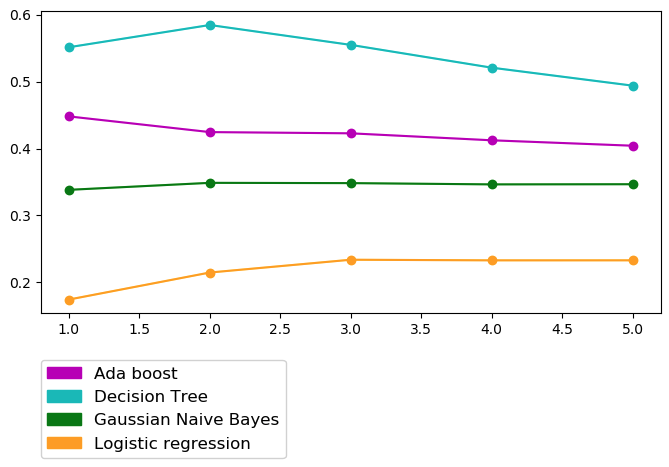
\includegraphics[width=12cm]{Immagini/mlTest.png}
		\caption{Accuratezze ottenute dai modelli addestrati. Sulle ascisse abbiamo il numero di PoS tag circostanti considerato, sulle ordinate l'accuratezza ottenuta}
		\label{fig:mlTest}
	\end{figure}
	
	Nel grafico in \autoref{fig:mlTest} abbiamo riportato sulle ascisse il valore di \texttt{PREVTAG} utilizzato, che ricordiamo abbiamo fatto coincidere con quello di \texttt{NEXTTAG}. Sulle ordinate abbiamo il valore di accuratezza corrispondente.\\
	Dunque a titolo d'esempio, il modello decision tree quando va a considerare i due PoS tag precedenti e i due PoS tag successivi, riesce ad individuare il PoS tag della parola compresa fra di essi nel $58\%$ dei casi.
\end{enumerate}

Per poter effettuare un confronto, in questo caso potremmo considerare come baseline il valore ottenuto andando a classificare sempre il tag corrente con il tag più frequente. Tale tag è il nome che si presenta nel $19\%$ dei casi.\\
Purtroppo le accuratezze ottenute mediante il modello logistic regression superano di poco -e non sempre superano!- il valore di baseline.\\
I risultati ottenuti dai modelli Gaussian naive Bayes e Ada boost sono invece intermedi, visto che si attestano tra il $35\%$ e il $45\%$.\\
\\
I risultati migliori sono quelli ottenuti mediante il modello decision tree. In questo caso il modello raggiunge punte di accuratezza del $55\%-58\%$.\\
In conclusione, i risultati ottenuti ci permettono di affermare che:
\begin{itemize}
	\item Non possiamo dire che sia sempre possibile determinare il PoS tag di una certa parola andando a considerare soltanto i PoS tag circostanti
	\item Ad ogni modo il fatto che un algoritmo di machine learning riesca ad individuare il PoS tag nel $58\%$ dei casi conferma l'esistenza di una struttura del linguaggio su cui è possibile effettuare apprendimento per determinare in alcuni casi il giusto PoS tag.  
\end{itemize}

\end{document}
